%% encoding: UTF-8
%% 首先读取模板的配置
% !Mode:: "TeX:UTF-8"
\PassOptionsToPackage{table}{xcolor}
\documentclass[12pt,openright]{book}
\usepackage[a4paper,
  bindingoffset=1cm,
  left=2.5cm, %2.5
  right=2.5cm,%2.5
  top=3cm,
  bottom=4cm,
  footskip=1.5cm,
  twoside]{geometry}

\usepackage[square,super,comma,sort]{natbib}
%\setcitestyle{open={\ensuremath{^[}},close={\ensuremath{^]}}}
\usepackage{float}
\usepackage{calc}
\usepackage[font={bf},labelsep=quad]{caption}
\usepackage{amsmath}
\usepackage{amsfonts}
%\usepackage{verbatim}
\usepackage{makecell}
\usepackage{tikz}
\usetikzlibrary{%
    arrows,%
    shapes,%
    chains,%
    matrix,%
    positioning,%
    scopes%
}
\usepackage{calc}
\usepackage{doc}
\usepackage{setspace}
\onehalfspacing
%\doublespacing
\parskip 0.5\baselineskip
\usepackage{ifthen}
% set linkcolor to blue for ebook :)

%\usepackage[dvipdfmx,bookmarks=true,bookmarksnumbered=false,
%            colorlinks,linkcolor=black,
%            citecolor=black,urlcolor=black]{hyperref}

% 2013-1-8,删去dvipdfmx
\usepackage[bookmarks=true,bookmarksnumbered=false,
            colorlinks,linkcolor=black,
            citecolor=black,urlcolor=black]{hyperref}

%\usepackage[dotinlabels]{titletoc}
\usepackage{fancyhdr}
\pagestyle{fancy}
\setlength\headheight{15pt}
%\fancyhf{}
%\fancyhead{\thepage}
% 2013-1-8 请在这里设置奇数偶数页的页眉格式
%\fancyhead[LE,RO]{\thepage}
%\fancyhead[RE,LO]{\thesection}
%\fancyhead[RE,LO]{\XMUT@value@title }
\usepackage{multirow}
\usepackage{longtable}
\usepackage{arydshln}
\setlength\dashlinedash{5pt}
\setlength\dashlinegap{2pt}
\newcommand*{\dd}[1]{\,\ensuremath{\mathrm{d}#1}}
\newcommand*{\ddd}[2]{\,\ensuremath{\mathrm{d}#1\mathrm{d}#2}}
\newcommand*{\dddd}[3]{\,\ensuremath{\mathrm{d}#1\mathrm{d}#2\mathrm{d}#3}}
\usepackage{txfonts}
%\usepackage{mathptmx}
\usepackage{fontspec}
\setmainfont[Mapping=tex-text]{Times New Roman PS Std}
\setsansfont[Mapping=tex-text]{Mosquito Formal Std}
%\setsansfont[Mapping=tex-text]{Myriad Pro}
\setmonofont[Scale=0.8]{Lucida Sans Typewriter Std}

\usepackage{xunicode}
\usepackage{xltxtra}

%\usepackage{mathspec}
%\setmathsfont[Set=Latin]{Asana Math}
%\setmathsfont[Set=Greek]{Asana Math}
%\setmathsfont[Set=Symbols]{Asana Math}
\usepackage{indentfirst}
\usepackage{zhspacing}
\usepackage[fakebold]{zhfont}
% for chinese font:
\newfontfamily\zhpunctfont{Adobe Song Std}
\setzhmainfont{Adobe Song Std}
\setzhsansfont{Adobe Heiti Std}
\setzhmonofont{Adobe Kaiti Std}
% for Chinese Numbers :)
\usepackage{config/xCJKnumb}

\renewcommand\chaptermark[1]
{\markboth{第\xCJKnumber{\thechapter}章\hspace{2ex} #1}{}}
\renewcommand\sectionmark[1]
{\markright{\thesection\quad #1}}
% redefine names
%\newcommand\contentsname{Contents}
\renewcommand\contentsname{目\quad{}录}
\newcommand\econtentsname{Contents}
\renewcommand\listfigurename{插图目录}
\renewcommand\listtablename{表格目录}
\renewcommand\bibname{参考文献}
\renewcommand\indexname{索引}
\renewcommand\figurename{图}
\renewcommand\tablename{表}
\renewcommand\partname{部分}
\renewcommand\appendixname{附录}
% read common comands
%% common definitions both for main and cover
%
%%%%%%%%%%%%%%%%%%%%%%%%%%%%%%%%%%%%%%%%%%%%%%%%%%%%%%%%%%%
% 重定义字号命令
%%%%%%%%%%%%%%%%%%%%%%%%%%%%%%%%%%%%%%%%%%%%%%%%%%%%%%%%%%%

\newcommand{\xiaochu}{\fontsize{30pt}{40pt}\selectfont}    % 小初, 1.5倍行距
\newcommand{\yihao}{\fontsize{26pt}{36pt}\selectfont}    % 一号, 1.4倍行距
\newcommand{\erhao}{\fontsize{22pt}{28pt}\selectfont}    % 二号, 1.25倍行距
\newcommand{\xiaoer}{\fontsize{18pt}{18pt}\selectfont}    % 小二, 单倍行距
\newcommand{\sanhao}{\fontsize{16pt}{24pt}\selectfont}    % 三号, 1.5倍行距
\newcommand{\xiaosan}{\fontsize{15pt}{22pt}\selectfont}    % 小三, 1.5倍行距
\newcommand{\sihao}{\fontsize{14pt}{21pt}\selectfont}    % 四号, 1.5倍行距
\newcommand{\banxiaosi}{\fontsize{13pt}{19.5pt}\selectfont}    % 半小四, 1.5倍行距
\newcommand{\xiaosi}{\fontsize{12pt}{18pt}\selectfont}    % 小四, 1.5倍行距
\newcommand{\dawuhao}{\fontsize{11pt}{11pt}\selectfont}    % 大五号, 单倍行距
\newcommand{\wuhao}{\fontsize{10.5pt}{10.5pt}\selectfont}    % 五号, 单倍行距
\newcommand{\xiaowu}{\fontsize{9pt}{9pt}\selectfont}    % 小五号, 单倍行距

\makeatletter
%% fill parbox to given width
\newlength{\@fillparboxlen}
\newcommand\fillparbox[2]{%
  \settowidth{\@fillparboxlen}{#2}
  \parbox[t]{\ifdim#1>\@fillparboxlen#1\else\@fillparboxlen\fi}{\hbadness 10000%
    \noindent\parfillskip 0pt #2}}
\newcommand\classification[1]{\def\XMUT@value@classification{#1}}
\newboolean{XMUT@boolean@confidential}
\newcommand\confidential[2]{\def\XMUT@value@confidential{#1}%
  \ifthenelse{\boolean{#2}}
    {\setboolean{XMUT@boolean@confidential}{true}}
    {\setboolean{XMUT@boolean@confidential}{false}}}
\newcommand\confidentialdate[3]{%
  \def\XMUT@value@confidentialdate@year{#1}%
  \def\XMUT@value@confidentialdate@month{#2}%
  \def\XMUT@value@confidentialdate@day{#3}}
\newcommand\UDC[1]{\def\XMUT@value@UDC{#1}}
\newcommand\serialnumber[1]{\def\XMUT@value@serialnumber{#1}}
\newcommand\studentsn[1]{\def\XMUT@value@studentsn{#1}}
\newcommand\school[1]{\def\XMUT@value@school{#1}}
\newcommand\degree[1]{%
  \def\XMUT@value@degree{#1}%
  \hypersetup{pdfsubject={厦门大学#1学位论文}}}
\renewcommand\title[2]{%
  \def\XMUT@value@title{#1}
  \def\XMUT@value@englishtitle{#2}
  \hypersetup{pdftitle={#1}}}
\renewcommand\author[1]{\def\XMUT@value@author{#1}
	\hypersetup{pdfauthor={#1}}}
\newcommand\advisor[2]{\def\XMUT@value@advisor{#1}%
    \def\XMUT@value@advisortitle{#2}}
\newcommand\major[1]{\def\XMUT@value@major{#1}}
\newcommand\submitdate[2]{%
  \def\XMUT@value@submitdate@year{#1}%
  \def\XMUT@value@submitdate@month{#2}}
  %\def\XMUT@value@submitdate@day{#3}}
\newcommand\defenddate[2]{%
  \def\XMUT@value@defenddate@year{#1}%
  \def\XMUT@value@defenddate@month{#2}}
  %\def\XMUT@value@defenddate@day{#3}}
\newcommand\grantdate[2]{%
  \def\XMUT@value@grantdate@year{#1}%
  \def\XMUT@value@grantdate@month{#2}}
  %\def\XMUT@value@grantdate@day{#3}}
\newcommand\chairman[1]{\def\XMUT@value@chairman{#1}}
\newcommand\appraiser[1]{\def\XMUT@value@appraiser{#1}}
\newcommand\team[1]{\def\XMUT@value@team{#1}}
\newcommand\fundteam[1]{\def\XMUT@value@fundteam{#1}}
\newcommand\lab[1]{\def\XMUT@value@lab{#1}}
%% add pdfkeywords, because this step must be done before \maketitle,
%% so we could not use the \keywords command in abstract.
\newcommand\pdfkeywords[1]{%
  \hypersetup{pdfkeywords={#1}}}
%
\makeatother


% start more DIY
\makeatletter
% for natbib
\renewcommand\NAT@citesuper[3]{\ifNAT@swa
\if*#2*\else#2\ \fi
\unskip\kern\p@\textsuperscript{\NAT@@open#1\NAT@@close}%
   \if*#3*\else\ #3\fi\else #1\fi\endgroup}

\renewcommand\textsuperscript[1]{\mbox{$^{\mbox{\scriptsize#1}}$}}
% for chapter
\newcommand\@chaplable[1]{第\xCJKnumber{#1}章}
\renewcommand\chapter{\if@openright\cleardoublepage\else\clearpage\fi
                    \thispagestyle{plain}%
                    \global\@topnum\z@
                    \@afterindentfalse
                    \secdef\@chapter\@schapter}
\renewcommand\@chapter[3][default]{%
                    \ifnum \c@secnumdepth >\m@ne
                       \if@mainmatter
                         \refstepcounter{chapter}%
                         \typeout{第\thechapter 章}%
                         \addcontentsline{toc}{chapter}%
                            {\protect\numberline{\@chaplable{\thechapter}}\hspace{-1.1em}#1}%
                         \addcontentsline{eoc}{chapter}%
                         {\protect\numberline{\textsc{\chaptername}\ \thechapter}#3}%
                       \else
                         \addcontentsline{toc}{chapter}{#1}%
                         \addcontentsline{eoc}{chapter}{#3}%
                       \fi
                    \else
                      \addcontentsline{toc}{chapter}{#1}%
                      \addcontentsline{eoc}{chapter}{#3}%
                    \fi
                    \chaptermark{#1}%
                    \addtocontents{lof}{\protect\addvspace{10\p@}}%
                    \addtocontents{lot}{\protect\addvspace{10\p@}}%
                    \if@twocolumn
                      \@topnewpage[\@makechapterhead{#2}]%
                    \else
                      \@makechapterhead{#2}%
                      \@afterheading
                    \fi}
\def\@makechapterhead#1{%
  \vspace*{10\p@}%
  {\parindent \z@ \raggedright \normalfont
    \ifnum \c@secnumdepth >\m@ne
      \if@mainmatter
        \centering \sffamily \bfseries \xiaosan  \@chaplable{\thechapter}\hspace{2ex}
      \fi
    \fi
    \interlinepenalty\@M
    #1\par\nobreak
    \vskip 10\p@
  }}

\def\@schapter#1{%
  \if@twocolumn
    \@topnewpage[\@makeschapterhead{#1}]%
  \else
    \@makeschapterhead{#1}%
    \@afterheading
  \fi%
}

\def\@makeschapterhead#1{%
  \vspace*{10\p@}%
  {\parindent \z@ \raggedright
    \interlinepenalty\@M
    \centering \sffamily \bfseries \xiaosan #1\par\nobreak
    \vskip 10\p@
  }%
}

\renewcommand*\l@chapter[2]{%
  \ifnum \c@tocdepth >\m@ne
    \addpenalty{-\@highpenalty}%
    \vskip 1.0em \@plus\p@
    \setlength\@tempdima{7em}%
    \begingroup
      \parindent \z@ \rightskip \@pnumwidth
      \parfillskip -\@pnumwidth
      \leavevmode \sffamily\bfseries\sihao
      \advance\leftskip\@tempdima
      \hskip -\leftskip
      #1\nobreak\hfil \nobreak\hb@xt@\@pnumwidth{\hss\rmfamily #2}\par
      \penalty\@highpenalty
    \endgroup
  \fi%
}
\renewcommand*\l@section[2]{\@dottedtocline{1}{1.5em}{2.3em}%
  %% {\sffamily\bfseries\xiaosi #1}{#2}} %% william: section 标题加粗
  {\sffamily\xiaosi #1}{#2}}
\renewcommand*\l@subsection[2]{\@dottedtocline{2}{3.8em}{3.2em}%
  %% {\rmfamily\bfseries\xiaosi #1}{#2}} %% william
  {\rmfamily\xiaosi #1}{#2}}
% for section
\renewcommand\section[2]{%
  \refstepcounter{section}
  \addcontentsline{toc}{section}%
    {\protect\numberline{\thesection}#1}%
  \addcontentsline{eoc}{section}%
    {\protect\numberline{\thesection}#2}%
  \sectionmark{#1}%
  \par\vspace{3.5ex \@plus 1ex \@minus -.2ex}%
  {%
    \parindent \z@ \raggedright
    \interlinepenalty\@M
   %%  \sffamily \bfseries \sihao \thesection \hspace{1em}#1\par\nobreak% % william
    \sffamily \sihao \thesection \hspace{1em}#1\par\nobreak%
  }%
  \vspace{2.3ex \@plus 0.2ex}
}
%
\renewcommand\subsection[2]{%
  \refstepcounter{subsection}
  \addcontentsline{toc}{subsection}%
    {\protect\numberline{\thesubsection}#1}%
  \addcontentsline{eoc}{subsection}%
    {\protect\numberline{\thesubsection}#2}%
  \par\vspace{3.25ex\@plus 1ex \@minus -.2ex}%
  {%
    \parindent \z@ \raggedright
    \interlinepenalty\@M
    %% \sffamily \bfseries \xiaosi \thesubsection \hspace{1em}#1\par\nobreak%  %% william
    \sffamily  \xiaosi \thesubsection \hspace{1em}#1\par\nobreak%
  }%
  \vspace{1.5ex \@plus 0.2ex}
}
%
\renewcommand\subsubsection{\@startsection{subsubsection}{3}{\z@}%
                                     {-3.25ex\@plus -1ex \@minus -.2ex}%
                                     {1.5ex \@plus .2ex}%
                                     %% {\sffamily\bfseries\xiaosi}}  %%william
                                     {\sffamily\xiaosi}}
%

\renewcommand\cleardoublepage{\clearpage\if@twoside \ifodd\c@page\else
  \thispagestyle{empty}%
  \hbox{}\newpage\if@twocolumn\hbox{}\newpage\fi\fi\fi}
  
%%用于产生没有编号但在目录中列出的章。
%% \phantomsection is the anchor hyperref needed to make a bookmark,
%% without it, hyerref would throw out warnings.
%% typeset Chinese Chapter, then list it in toc and eoc
\newcommand\CNchapter[2]{%
  \chapter*{\phantomsection %
  \center{#1}}%
  \markboth{#1}{}%
  \addcontentsline{toc}{chapter}{#1}%
  \addcontentsline{eoc}{chapter}{#2}%
}
%% typeset English Chapter, then list it in toc and eoc
\newcommand\ENchapter[2]{%
  \chapter*{\phantomsection %
  \center{#2}}%
  \markboth{#2}{}%
  \addcontentsline{toc}{chapter}{#1}%
  \addcontentsline{eoc}{chapter}{#2}%
}
%% Chinese Chapter only in toc
\newcommand\Cchapter[1]{%
  \chapter*{\phantomsection %
    \center{#1}}%
  \markboth{#1}{}%
  \addcontentsline{toc}{chapter}{#1}%
}
%% English Chapter only in eoc
\newcommand\Echapter[1]{%
  \chapter*{\phantomsection %
  \center{#1}}%
  \markboth{#1}{}%
  \addcontentsline{eoc}{chapter}{#1}%
}
%

%%============================摘要===========================%%

%%中文摘要。
\newenvironment{abstract}
  {\Cchapter{\texorpdfstring{摘\quad 要}{摘要}}
  \pagenumbering{Roman}
  \setcounter{page}{1}}
  {}
%%中文关键词。
\newcommand\keywords[1]{%
  \vspace{2ex}\noindent{\sffamily \bfseries 关键词:} #1}

  
%%英文摘要。
\newenvironment{englishabstract}
  {\ENchapter{英文摘要}{Abstract}%
  \parindent 0pt}
  {}
%%英文关键词。
\newcommand\englishkeywords[1]{%
  \vspace{2ex}\noindent{\sffamily \bfseries Keywords:} #1}

%% Thanks
\renewenvironment{thanks}
  {\CNchapter{\texorpdfstring{致\quad{}谢}{致谢}}{Thanks}}
  {\ifodd\c@page%
    \newpage\thispagestyle{empty}
    \hbox{}\fi }
%% publications, options is the number of publications
\newenvironment{publications}[1]
  {\CNchapter{\XMUT@value@degree 期间发表的论文}{Publications as the Degree Candidate}%
    \list{\@biblabel{\@arabic\c@enumi}}%
      {\settowidth\labelwidth{\@biblabel{#1}}%
        \leftmargin\labelwidth
        \advance\leftmargin\labelsep
        \@openbib@code
        \usecounter{enumi}%
        \let\p@enumi\@empty
        \renewcommand\theenumi{\@arabic\c@enumi}}%
    \sloppy
    \clubpenalty4000
    \@clubpenalty \clubpenalty
    \widowpenalty4000%
    \sfcode`\.\@m}
 {\def\@noitemerr
   {\@latex@warning{Empty `publications' environment}}%
  \endlist}

%%======================参考文献======================%%

%%修改thebibliography 的定义以在目录中加入相应条目。
\renewenvironment{thebibliography}[1]
  {\CNchapter{\bibname}{References}%
	  \@mkboth{\MakeUppercase\bibname}{\MakeUppercase\bibname}%
	  \wuhao%用比正文小一号的字体排印参考文献内容
	  \list{\@biblabel{\@arabic\c@enumiv}}%
		   {\settowidth\labelwidth{\@biblabel{#1}}%
			\leftmargin\labelwidth
			\advance\leftmargin\labelsep
			\@openbib@code
			\usecounter{enumiv}%
			\let\p@enumiv\@empty
			\renewcommand\theenumiv{\@arabic\c@enumiv}}%
	  \sloppy
	  \clubpenalty4000
	  \@clubpenalty \clubpenalty
	  \widowpenalty4000%
	  \sfcode`\.\@m}
	 {\def\@noitemerr
	   {\@latex@warning{Empty `thebibliography' environment}}%
	  \endlist}

%%===========================目录==============================%%

%%设置目录格式。
\renewcommand\tableofcontents{%
    \if@twocolumn
      \@restonecoltrue\onecolumn
    \else
      \@restonecolfalse
    \fi
    \begingroup
    \parskip 0pt
    \Cchapter{\texorpdfstring{\contentsname}{目录}}%
    \@starttoc{toc}%
    %\ENchapter{英文目录}{\econtentsname}%
    %\@starttoc{eoc}%
    \endgroup
    \if@restonecol\twocolumn\fi%
    \cleardoublepage%
    }

%%====================封面==========================
\newcommand\underlinewidth[2][50pt]{\underline{\parbox[t]{#1}{\centering#2}}}
%
\renewcommand\maketitle{%
  \begin{titlepage}
    \addtolength{\oddsidemargin}{-0.5cm}
    \begin{center}
      \parskip 0pt
      \vskip \stretch{2}
      
\includegraphics[width=5.8cm]{figures/xmu-zi-3d-600dpi}\\
      \vskip \stretch{0.5}
      {\rmfamily\bfseries\xiaoer
        \fillparbox{198pt}{%\XMUT@value@degree%
        王亚南经济研究院}\\
      }
      \vskip \stretch{2}
      
\rule{\textwidth}{1pt}\par % Thick horizontal line
\vspace{2pt}\vspace{-\baselineskip} % Whitespace between lines
\rule{\textwidth}{0.4pt}\par % Thin horizontal line
\vskip \stretch{.5}

        {\sffamily\bfseries
          \erhao \textcolor{red}{\XMUT@value@title}
        }
      \vskip \stretch{.5}
        {\rmfamily\bfseries
          \sanhao \textcolor{red}{\XMUT@value@englishtitle}
        }
        
\rule{\textwidth}{1pt}\par % Thick horizontal line
\vspace{2pt}\vspace{-\baselineskip} % Whitespace between lines
\rule{\textwidth}{0.4pt}\par % Thin horizontal line
\vskip \stretch{.5}

      \vskip \stretch{2}
      \newlength{\XMUT@len@author}
      \settowidth{\XMUT@len@author}{\XMUT@value@author}
      \setlength{\XMUT@len@author}{\XMUT@len@author * \real{1.8}}
        {\ttfamily\mdseries\xiaoer
          \fillparbox{\XMUT@len@author}{\XMUT@value@author}
        }          
      \vskip \stretch{1}
      \vspace{-2cm}
      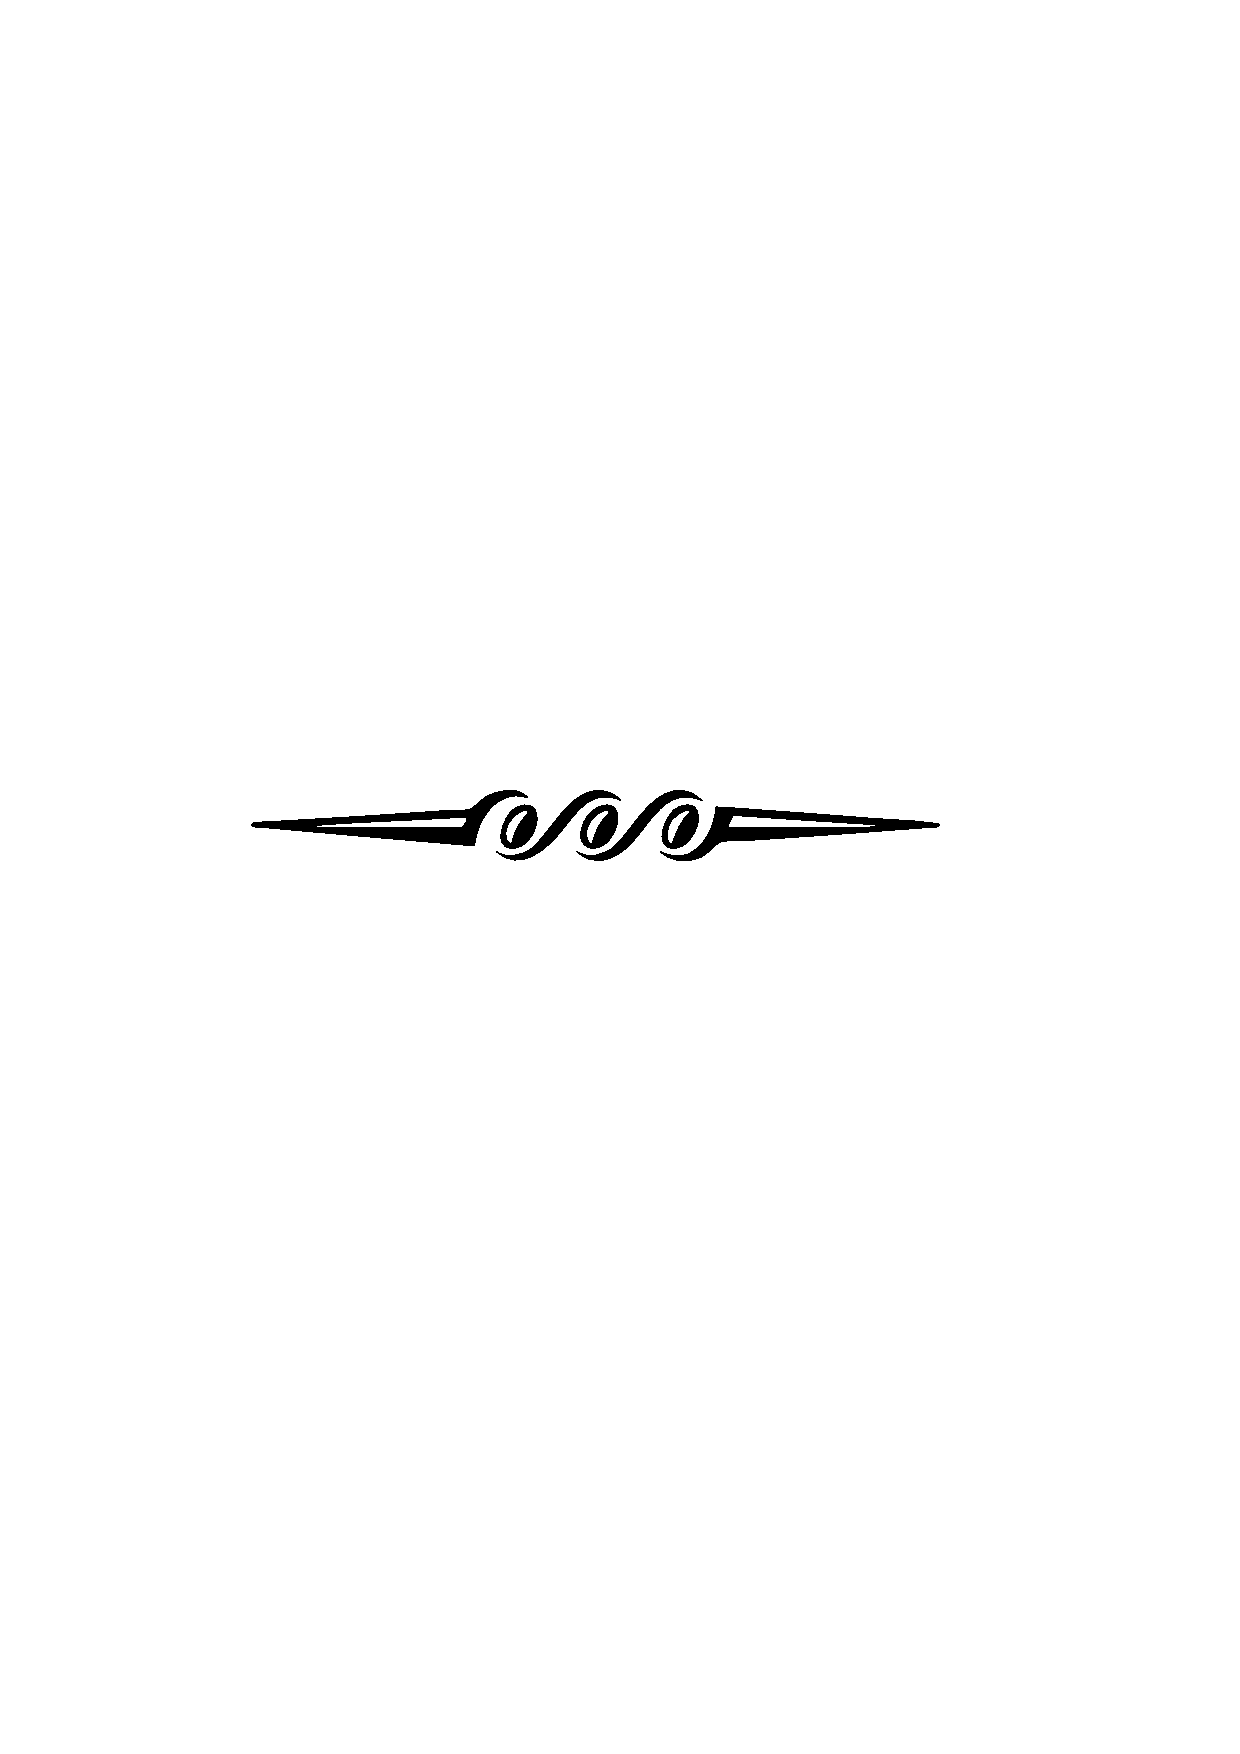
\includegraphics[scale=.3]{figures/blackbase}
      %\def\tabcolsep{1pt}
      %\def\arraystretch{1.5}
      \newlength{\XMUT@len@advisor}
      \settowidth{\XMUT@len@advisor}{\XMUT@value@advisor\hspace*{1.5em}\XMUT@value@advisortitle}
      %% length for ~~
      %\addtolength{\XMUT@len@advisor}{30pt}
      \setlength{\XMUT@len@advisor}{\ifdim \XMUT@len@advisor > 84pt \XMUT@len@advisor
        \else 84pt
        \fi}
      \vskip \stretch{2}
    \end{center}
  \end{titlepage}
  %\cleardoublepage
  % 版权声明
  %\clearpage
}
\makeatother
%---------------------------- 数学公式设置 ------------------------------%
%\setlength{\abovedisplayskip}{6pt plus1pt minus1pt}     %公式前的距离
%\setlength{\belowdisplayskip}{6pt plus1pt minus1pt}     %公式后面的距离
\setlength{\arraycolsep}{4pt}   %在一个array中列之间的空白长度, 因为原来的太宽了

% \eqnarray如果很长,影响分栏、换行和分页(整块挪动,造成页面空白),
% 可以设置成为自动调整模式
\allowdisplaybreaks[4]

%%%%%%%%%%%%%%%%%%%%%%%%%%%%%%%%%%%%%%%%%%%%%%%%%%%%%%%%%%%
%下面这组命令使浮动对象的缺省值稍微宽松一点,从而防止幅度
%对象占据过多的文本页面,也可以防止在很大空白的浮动页上放置
%很小的图形。
%%%%%%%%%%%%%%%%%%%%%%%%%%%%%%%%%%%%%%%%%%%%%%%%%%%%%%%%%%%
\renewcommand{\textfraction}{0.15}
\renewcommand{\topfraction}{0.85}
\renewcommand{\bottomfraction}{0.65}
\renewcommand{\floatpagefraction}{0.80}

\pagenumbering{roman}


\begin{document}
%% 确保zhspacing需要的符号定义没有被其他宏包改掉
\def\lq{`}\def\rq{'} 
\zhspacing

%% 读入作者的信息
% !Mode:: "TeX:UTF-8"
%% 中图分类号
\classification{T192}
%% 保密不?第一个参数是显示在封面上的,第二个参数是选择著作权使用声明中打哪个勾
\confidential{公开}{false}
%% 如果是保密论文,你可能想把保密日期一并填上
%\confidentialdate{2009}{9}{9}
\UDC{ }
\studentsn{27720101152678}
%\degree{硕士}
\author{方 莲}
\school{厦门大学}
\title{中恒通(福建)机械制造有限公司}
{\Huge 投资价值分析报告}
\advisor{牛霖琳}{教授}
\chairman{答辩主席}
\major{西方经济学}
\submitdate{2014}{3}
\defenddate{2014}{5}
\grantdate{2014}{7}
\appraiser{老师一~~老师二}

%% 用在原创性声明中的
\team{ }
\fundteam{ }
%\lab{化学化工学院~过程控制实验室}


%% 加入pdf文件的关键字,\pdfkeywords必须在\maketitle之前才有效
\pdfkeywords{XeLaTeX;厦门大学硕博学位论文模板}

%% 生成a4封面、原创性声明、著作权使用声明
\maketitle

%% 正文默认使用小四,字号的定义在 config/headcommon.tex中
\xiaosi

%% 读入中英文摘要
\begin{abstract}
中恒通(福建)机械制造有限公司(以下简称「中恒通」)由原始合伙人以共同认缴出资的方式于2008年3月获批正式成立,发展成为集科研、设计、生产、销售、贸易于一体汽车底盘制造商,目前主营业务涵盖商用车制动鼓、轮毂、工程机械桥壳、刹车盘、刹车片等载重汽车底盘零部件。为了便于投资者加强对该公司的生产运作、经营管理、财务状况等有企业情况的深入了解,本报告将依据目前中恒通已经披露的2013年度和2012年度财务报表,对该公司的情况进行客观翔实的分析,并向投资者提示目前存在的主要投资风险等。

投资有风险。本报告仅为分析员个人观点,不构成对中恒通的任何投资建议。

\keywords{中恒通;财务报表;股权投资;资本运作}
\end{abstract}


\begin{englishabstract}
    Here is your English Abstract.

\englishkeywords{keyword1; keyword2; keyword3}
\end{englishabstract}

%% 生成中英文目录
\tableofcontents

%% 以数字风格开始正文页码
\pagenumbering{arabic}

%% 读入各章节
\chapter{简要的说明}{Introduction}

    这个模板是本人在完成硕士论文时做的,幸运的是在我之前已经有不少人做了
    一些不错的厦大论文\LaTeX{}模板使我的进展快了不少。之所以写这个模板是
    因为\XeLaTeX{}能够很方便地支持中英文混排有相当一段时间了,但现有的模
    板依然是基于数年前北京大学的\LaTeX{}模板做的。
    秉承自强不息,止于至善的校训,我就DIY了一把。

    在模板的编写中,朱建平教授\citep{zhujianpin:2009}的\LaTeX{}模板以及陈昱\citep{chenyu:2005}的XMUThesis模板给了我
    很大的启发。而\LaTeX{} Companion II\citep{latexcompii}和\LaTeX{}实用教程\citep{latexguide}是整天翻阅的参考书籍。
    原以为一切都OK的时候把在论文拿去打印才发现打印店需要A3+(440mm x 297mm)的封面,汗了一把赶紧马上研究A3的封面制作。
    此时,东南大学的学位论文模板\citep{seu:latex}给我了很大的启发,使我在2个小时内
    折腾出了第一个可用的A3封面模板。
    对完成以上各个模板的前人们一都表示我衷心的谢意 :)

    模板是仓促完成的,虽然已经实际用在了我的论文中,但难免有不足和疏漏。
    各位在使用中如发现什么bug或建议请直接email联系我:acevery@gmail.com。

    \hfill 余钰炜

\chapter{示例}{Examples}
\section{用PGF画图}{Draw with PGF}
PGF\citep{tantau:pgf}是非常强大的\LaTeX{}画图宏包,必须承认本人较有洁癖,
加上做的课题没有实验截图,所以整篇论文中的图都是用PGF画的矢量图形。下面主要给出一些论文中
用PGF画图的示例,希望对使用者有所帮助。PGF详细具体的说明请查阅PGF自带的手册,做完里面的Tutorial后,
以各位的高智商应该可以轻松运用了。

当然阁下可以选择方便地插入位图,具体的步骤网上一抓无数,这里就不重复劳动了。

图\ref{fig:mexican_hat}是用PGF+GNUPlot画出墨西哥小波函数的例子。注意,plot file命令中的“/”
是Linux下的路径分隔符,如果你是在Windows下的话需要改为“\textbackslash ”才可以的哦。
\small{
\begin{verbatim}
\begin{figure}[htpb]
    \begin{center}
        \begin{tikzpicture}[>=stealth,thick]
            \draw [->] (-5.5,0) -- (6,0);
            \draw [->] (0, -2.5) -- (0, 5);
            \draw [color=blue] plot file {figures/gnuplot/mexican.table};
            \draw node at (0,0) [below left, color=gray] {$O$};
            \foreach \x in {-5,-4,-3,-2,-1, 1, 2, 3, 4, 5}
                \draw (\x, 1pt) -- (\x, -1pt) node [below=2pt,color=gray] {$\x$};
        \node at (6,0) [below=4pt, color=gray] {$x$};
            \foreach \y/\yy in {-2/-0.2, -1/-0.1, 1/0.1, 2/0.2, 3/0.3, 4/0.4}
                \draw (-1pt, \y) -- (1pt, \y) node [left=6pt,color=gray] {$\yy$};
        \node at (0,5) [left=6pt, color=gray] {$y$};
        \end{tikzpicture}
    \end{center}
    \caption{Mexican Hat Wavelet}
    \label{fig:mexican_hat}
\end{figure}
\end{verbatim}
}

\begin{figure}[htpb]
    \begin{center}
        \begin{tikzpicture}[>=stealth,thick]
            \draw [->] (-5.5,0) -- (6,0);
            \draw [->] (0, -2.5) -- (0, 5);
            \draw [color=blue] plot file {figures/gnuplot/mexican.table};
            \draw node at (0,0) [below left, color=gray] {$O$};
            \foreach \x in {-5,-4,-3,-2,-1, 1, 2, 3, 4, 5}
                \draw (\x, 1pt) -- (\x, -1pt) node [below=2pt,color=gray] {$\x$};
	    \node at (6,0) [below=4pt, color=gray] {$x$};
            \foreach \y/\yy in {-2/-0.2, -1/-0.1, 1/0.1, 2/0.2, 3/0.3, 4/0.4}
                \draw (-1pt, \y) -- (1pt, \y) node [left=6pt,color=gray] {$\yy$};
	    \node at (0,5) [left=6pt, color=gray] {$y$};
        \end{tikzpicture}
    \end{center}
    \caption{Mexican Hat Wavelet}
    \label{fig:mexican_hat}
\end{figure}

当然,我们往往需要画出一些数据处理的示意图,如图\ref{fig:dwt_idwt},就是小波分解和合成的简要示意。
\small{
\begin{verbatim}
\begin{figure}[htpb]
    \begin{center}
        \begin{tikzpicture}[>=stealth]
            \draw [->] (0.3,0) -- (1,0) -- (1,0.6) -- (1.5,0.6);
            \draw node at (0.3,0) [left] {$v(t)$};
            \draw [->] (1.5,0.6) -- (5, 0.6);
            \draw node at (4.3, 0.6) [above] {$c_{jk}$};
            \draw [->] (1,0) -- (1,-0.6) -- (1.5,-0.6);
            \draw [->] (1.5,-0.6) -- (5,-0.6);
            \draw node at (4.3, -0.6) [above] {$d_{jk}$};
            \draw node at (1.5,0.6) [right,rectangle,draw,fill=white] {$\langle
            v(t) | \phi_{jk}(t)\rangle$};
            \draw node at (1.5,-0.6) [right,rectangle,draw,fill=white] {$\langle
            v(t) | \psi_{jk}(t)\rangle$};
            \draw (5,-1.2) rectangle ++ (4.2, 2.4);
            \draw node at (5.5, 0.6) [right] {$\sum c_{Jk}\phi_{Jk}(t)$};
            \draw node at (5.5, -0.6) [right] {$\sum\sum d_{jk}\psi_{jk}(t)$};
            \draw [->] (8,0.6) -- (8.5,0.6) -- ++(0,-0.3);
            \draw [->] (8,-0.6) -- (8.5,-0.6) -- ++(0,0.3);
            \draw (8.5,0) circle (0.3) node {+};
            \draw [->](8.8,0) -- (9.8,0) node [right] {$v(t)$};
        \end{tikzpicture}
    \end{center}
    \caption{离散小波分解与小波合成}
    \label{fig:dwt_idwt}
\end{figure}
\end{verbatim}
}
\begin{figure}[htpb]
    \begin{center}
        \begin{tikzpicture}[>=stealth]
            \draw [->] (0.3,0) -- (1,0) -- (1,0.6) -- (1.5,0.6);
            \draw node at (0.3,0) [left] {$v(t)$};
            \draw [->] (1.5,0.6) -- (5, 0.6);
            \draw node at (4.3, 0.6) [above] {$c_{jk}$};
            \draw [->] (1,0) -- (1,-0.6) -- (1.5,-0.6);
            \draw [->] (1.5,-0.6) -- (5,-0.6);
            \draw node at (4.3, -0.6) [above] {$d_{jk}$};
            \draw node at (1.5,0.6) [right,rectangle,draw,fill=white] {$\langle
            v(t) | \phi_{jk}(t)\rangle$};
            \draw node at (1.5,-0.6) [right,rectangle,draw,fill=white] {$\langle
            v(t) | \psi_{jk}(t)\rangle$};
            \draw (5,-1.2) rectangle ++ (4.2, 2.4);
            \draw node at (5.5, 0.6) [right] {$\sum c_{Jk}\phi_{Jk}(t)$};
            \draw node at (5.5, -0.6) [right] {$\sum\sum d_{jk}\psi_{jk}(t)$};
            \draw [->] (8,0.6) -- (8.5,0.6) -- ++(0,-0.3);
            \draw [->] (8,-0.6) -- (8.5,-0.6) -- ++(0,0.3);
            \draw (8.5,0) circle (0.3) node {+};
            \draw [->](8.8,0) -- (9.8,0) node [right] {$v(t)$};
        \end{tikzpicture}
    \end{center}
    \caption{离散小波分解与小波合成}
    \label{fig:dwt_idwt}
\end{figure}

图\ref{fig:mra}是简单流程图的示意。
\small{
\begin{verbatim}
\begin{figure}[htpb]
    \begin{center}
        \begin{tikzpicture}[->,node distance=7mm and 5mm,>=stealth,
            mn/.style={
            rectangle,
            draw=white
            }]
            \node (LR) {$L^2(R)$};
            \node (VJ) [right=of LR]{$V_J$};
            \node (VJm1) [right=of VJ] {$V_{J-1}$};
            \node (WJm1) [below=of VJm1] {$W_{J-1}$};
            \node (dots) [right=of VJm1] {$\cdots$};
            \node (V1) [right=of dots] {$V_1$};
            \node (W1) [below=of V1] {$W_1$};
            \node (V0) [right=of V1] {$V_0$};
            \node (W0) [below=of V0] {$W_0$};
            \path (LR) edge (VJ)
            (VJ) edge (VJm1)
            (VJ) edge[in=150,out=330]  (WJm1)
            (VJm1) edge (dots)
            (dots) edge (V1)
            (dots) edge[in=150,out=330] (W1)
            (V1) edge (V0)
            (V1) edge [in=150,out=330] (W0)
            ;
        \end{tikzpicture}
    \end{center}
    \caption{多分辨分析示意图}
    \label{fig:mra}
\end{figure}
\end{verbatim}
}

\begin{figure}[htpb]
    \begin{center}
        \begin{tikzpicture}[->,node distance=7mm and 5mm,>=stealth,
            mn/.style={
            rectangle,
            draw=white
            }]
            \node (LR) {$L^2(R)$};
            \node (VJ) [right=of LR]{$V_J$};
            \node (VJm1) [right=of VJ] {$V_{J-1}$};
            \node (WJm1) [below=of VJm1] {$W_{J-1}$};
            \node (dots) [right=of VJm1] {$\cdots$};
            \node (V1) [right=of dots] {$V_1$};
            \node (W1) [below=of V1] {$W_1$};
            \node (V0) [right=of V1] {$V_0$};
            \node (W0) [below=of V0] {$W_0$};
            \path (LR) edge (VJ)
            (VJ) edge (VJm1)
            (VJ) edge[in=150,out=330]  (WJm1)
            (VJm1) edge (dots)
            (dots) edge (V1)
            (dots) edge[in=150,out=330] (W1)
            (V1) edge (V0)
            (V1) edge [in=150,out=330] (W0)
            ;
        \end{tikzpicture}
    \end{center}
    \caption{多分辨分析示意图}
    \label{fig:mra}
\end{figure}


图\ref{fig:mallat}所示是复杂一些的流程图。
\small{
\begin{verbatim}
\begin{figure}[htpb]
    \begin{center}
        \begin{tikzpicture}[node distance=5mm and 12mm,>=stealth,
            an/.style={
            rectangle,
            draw=black
            },
            pn/.style={coordinate},
            cn/.style={
            font=\small
            }
            ]
            \node (Vt) [an] {$V(t)$};
            \node (C2) [an, above right=of Vt]{$C_2$};
            \node (D2) [an, below right=of Vt]{$D_2$};
            \node (C1) [an, above right=of C2]{$C_1$};
            \node (D1) [an, below right=of C2]{$D_1$};
            \node (C0) [an, above right=of C1]{$C_0$};
            \node (D0) [an, below right=of C1]{$D_0$};
            \node (C1') [an, below right=of C0]{$C_1'$};
            \node (C2') [an, below right=of C1']{$C_2'$};
            \node (pC1') [pn,right=of D1,xshift=24mm] {};
            \node (VT') [an, below right=of C2']{$V(t)'$};
            \node (pC2') [pn,right=of D2,xshift=60mm] {};
            \path
                (Vt) edge [->,out=10, in=190] node[cn,left,pos=0.8] {$H, \downarrow2\,$} (C2)
                (Vt) edge [->,out=-10, in=-190] node[cn,left,pos=0.8] {$G, \downarrow2\,$} (D2)
                (C2) edge [->,out=10, in=190] node[cn,left,pos=0.8] {$H, \downarrow2\,$} (C1)
                (C2) edge [->,out=-10, in=-190] node[cn,left,pos=0.8] {$G, \downarrow2\,$} (D1)
                (C1) edge [->,out=10, in=190] node[cn,left,pos=0.8] {$H, \downarrow2\,$} (C0)
                (C1) edge [->,out=-10, in=-190] node[cn,left,pos=0.8] {$G, \downarrow2\,$} (D0)
                (C0) edge  [->,out=-10, in=-190] node[cn,right,pos=0.2] {$\,\uparrow2,H^*$} (C1')
                (D0) edge [->,out=0,in=190] node[cn,right,pos=0.2] {$\,\uparrow2,G^*$} (C1')
                (C1') edge  [->,out=-10, in=-190] node[cn,right,pos=0.2] {$\,\uparrow2,H^*$} (C2')
                (D1) edge node[cn,above,pos=0.6] {$\,\uparrow2,G^*$}(pC1')
                (pC1') edge [->,out=0,in=200]  (C2')
                (C2') edge  [->,out=-10, in=-190] node[cn,right,pos=0.2] {$\,\uparrow2,H^*$} (VT')
                (D2) edge node[cn,above,pos=0.57] {$\,\uparrow2,G^*$} (pC2')
                (pC2') edge [->,out=0,in=190] (VT')
            ;
        \end{tikzpicture}
    \end{center}
    \caption{Mallat塔式算法示意图}
    \label{fig:mallat}
\end{figure}
\end{verbatim}
}
\begin{figure}[htpb]
    \begin{center}
        \begin{tikzpicture}[node distance=5mm and 12mm,>=stealth,
            an/.style={
            rectangle,
            draw=black
            },
            pn/.style={coordinate},
            cn/.style={
            font=\small
            }
            ]
            \node (Vt) [an] {$V(t)$};
            \node (C2) [an, above right=of Vt]{$C_2$};
            \node (D2) [an, below right=of Vt]{$D_2$};
            \node (C1) [an, above right=of C2]{$C_1$};
            \node (D1) [an, below right=of C2]{$D_1$};
            \node (C0) [an, above right=of C1]{$C_0$};
            \node (D0) [an, below right=of C1]{$D_0$};
            \node (C1') [an, below right=of C0]{$C_1'$};
            \node (C2') [an, below right=of C1']{$C_2'$};
            \node (pC1') [pn,right=of D1,xshift=24mm] {};
            \node (VT') [an, below right=of C2']{$V(t)'$};
            \node (pC2') [pn,right=of D2,xshift=60mm] {};
            \path
                (Vt) edge [->,out=10, in=190] node[cn,left,pos=0.8] {$H, \downarrow2\,$} (C2)
                (Vt) edge [->,out=-10, in=-190] node[cn,left,pos=0.8] {$G, \downarrow2\,$} (D2)
                (C2) edge [->,out=10, in=190] node[cn,left,pos=0.8] {$H, \downarrow2\,$} (C1)
                (C2) edge [->,out=-10, in=-190] node[cn,left,pos=0.8] {$G, \downarrow2\,$} (D1)
                (C1) edge [->,out=10, in=190] node[cn,left,pos=0.8] {$H, \downarrow2\,$} (C0)
                (C1) edge [->,out=-10, in=-190] node[cn,left,pos=0.8] {$G, \downarrow2\,$} (D0)
                (C0) edge  [->,out=-10, in=-190] node[cn,right,pos=0.2] {$\,\uparrow2,H^*$} (C1')
                (D0) edge [->,out=0,in=190] node[cn,right,pos=0.2] {$\,\uparrow2,G^*$} (C1')
                (C1') edge  [->,out=-10, in=-190] node[cn,right,pos=0.2] {$\,\uparrow2,H^*$} (C2')
                (D1) edge node[cn,above,pos=0.6] {$\,\uparrow2,G^*$}(pC1')
                (pC1') edge [->,out=0,in=200]  (C2')
                (C2') edge  [->,out=-10, in=-190] node[cn,right,pos=0.2] {$\,\uparrow2,H^*$} (VT')
                (D2) edge node[cn,above,pos=0.57] {$\,\uparrow2,G^*$} (pC2')
                (pC2') edge [->,out=0,in=190] (VT')
            ;
        \end{tikzpicture}
    \end{center}
    \caption{Mallat塔式算法示意图}
    \label{fig:mallat}
\end{figure}

\section{表格}{Tables}
    表格一般可以用tabular、tabularx、longtable等环境,我自己的论文中只用到了longtable,所以下面
    就举个简单的例子。

\begin{longtable}[c]{llll}
    \caption{longtable示例}\\ \hline
        \textsf{项目1}&    \textsf{项目2}&    \textsf{项目3}&    \textsf{项目3}\\ \hline
    \endfirsthead
        \multicolumn{4}{r}{\footnotesize{续上页表\thetable}} \\
        \hline \textsf{项目1}&    \textsf{项目2}&    \textsf{项目3}&    \textsf{项目3}\\ \hline
    \endhead
        \hline \multicolumn{4}{r}{\footnotesize{表格接下页\ldots}}
    \endfoot
        \hline
    \endlastfoot
        拼命打字&    认真画图&    好好写程序&    早睡早起\\
        拼命打字&    认真画图&    好好写程序&    早睡早起\\
        拼命打字&    认真画图&    好好写程序&    早睡早起\\
        拼命打字&    认真画图&    好好写程序&    早睡早起\\
        拼命打字&    认真画图&    好好写程序&    早睡早起\\
        拼命打字&    认真画图&    好好写程序&    早睡早起\\
        拼命打字&    认真画图&    好好写程序&    早睡早起\\
        拼命打字&    认真画图&    好好写程序&    早睡早起\\
        拼命打字&    认真画图&    好好写程序&    早睡早起\\
        拼命打字&    认真画图&    好好写程序&    早睡早起\\
        拼命打字&    认真画图&    好好写程序&    早睡早起\\
        拼命打字&    认真画图&    好好写程序&    早睡早起\\
        拼命打字&    认真画图&    好好写程序&    早睡早起\\
        拼命打字&    认真画图&    好好写程序&    早睡早起\\
        拼命打字&    认真画图&    好好写程序&    早睡早起\\
        拼命打字&    认真画图&    好好写程序&    早睡早起\\
        拼命打字&    认真画图&    好好写程序&    早睡早起\\
        拼命打字&    认真画图&    好好写程序&    早睡早起\\
        拼命打字&    认真画图&    好好写程序&    早睡早起\\
        拼命打字&    认真画图&    好好写程序&    早睡早起\\
        拼命打字&    认真画图&    好好写程序&    早睡早起\\
        拼命打字&    认真画图&    好好写程序&    早睡早起\\
        拼命打字&    认真画图&    好好写程序&    早睡早起\\
        拼命打字&    认真画图&    好好写程序&    早睡早起\\
        拼命打字&    认真画图&    好好写程序&    早睡早起\\
        拼命打字&    认真画图&    好好写程序&    早睡早起\\
        拼命打字&    认真画图&    好好写程序&    早睡早起\\
        拼命打字&    认真画图&    好好写程序&    早睡早起\\
        拼命打字&    认真画图&    好好写程序&    早睡早起\\
        拼命打字&    认真画图&    好好写程序&    早睡早起\\
        拼命打字&    认真画图&    好好写程序&    早睡早起\\
\end{longtable}

\section{参考文献的加入}{Adding Bibliographies}
参考文献可以用Google的学术搜索获得\BibTeX{}的格式\citep{zhujianpin:2009}。首先打开Google的学术搜索,在搜索按钮边上有一个偏好设置的链接。进入后,在页面的最下角有一个Bibliography Manager,选择Show links to import 
into BibTeX。这样当你搜索到你要加入的文献的时候,点 Import to BibTeX就能打开一个已经完成的BibTeX条目了。当然,为了保证整体的英文名子风格统一,你需要检查一下作者英文名字的大小写、缩写是否和要求的一致。


%% 参考文献
\bibliographystyle{reference/xmuthesis2}
\bibliography{reference/reference}

%% 发表的论文
\begin{publications}{2} % 这里的2是发表刊物的数量,用于计算需要缩进的长度用
    \item 第一作者, 第二作者, 第三作者.
        文章名一.
        刊物, 2009, 08:10-13.
    \item 第一作者, 第二作者, 第三作者.
        文章名二.
        刊物, 2009, 09:20-23.

\end{publications}


%% 最后致谢一下
\begin{thanks}
    谢谢父母

    谢谢导师

    谢谢朋友

    谢谢同学

    谢谢其他人
\end{thanks}


\end{document}
